\documentclass{report}


\usepackage{bibgerm}
\usepackage[numbers,sort&compress]{natbib}
\usepackage{amsmath,amssymb,mathtools}
\usepackage{algpseudocode,algorithm}
\usepackage{graphicx}
\usepackage{hyperref}
\usepackage{multirow}
\usepackage[utf8]{inputenc}
\usepackage{geometry}
\usepackage{parskip}
\usepackage{paralist}
\usepackage{multicol}

\geometry{verbose,a4paper,tmargin=25mm,bmargin=25mm,lmargin=15mm,rmargin=20mm}

%% Stuff ist aus ML1. vllt brauchen wir es ja noch :D
\DeclareMathOperator*{\argmax}{arg\,max}
\DeclareMathOperator*{\argmin}{arg\,min}

\newcommand{\IndState}[1][1]{\State\hspace{10mm}}
\newcommand{\mparagraph}[1]{\paragraph{#1} \mbox{}\\}

%%%%%%%%%%%%%% includeonly %%%%%%%%%%%%%%%%%%%
% Es werden nur die Teile eingebunden, die hier
% aufgefuehrt sind!
%\include{Kapitel X}
%}um es anzuzeigen.
%%%%%%%%%%%%%%%%%%%%%%%%%%%%%%%%%%%%%%%%%%%%%%
\graphicspath{{pic/}}

\begin{document}

\tableofcontents


% einfach !TEX root = rob1.tex an den Anfang packen von chaptern
% !TEX root = rob1.tex
\chapter{Einführung}

\subsection{Begriffsbildung}

\mparagraph{Roboter}
\begin{compactitem}
    \item \textbf{Industrie}: Ein Roboter ist ein frei programmierbarer, multifunktionaler
    Manipulator mit mindenstes 3 unabhängigen Achsen, um Materialien, Teile, Werkzeuge oder
    Geräte auf programmierten, variablen Bahnen zu bewegen zur Erfüllung verschiedener Aufgaben.
    \item \textbf{Wissenschaft}: Roboter sind sensomotorische Maschinen zur Erweiterung der
    menschlichen Handlungsfähigkeit. Sie bestehen aus mechatronischen Komponenten, Sensoren und
    rechnerbasierten Kontroll- und Steuerungsfunktionen.
\end{compactitem}

\mparagraph{Robotik}
Robotik ist ein interdisziplinär ausgerichtetes Forschungsgebiet, bei dem im Mittelpunkt mechanische
Vorrichtungen und geeignete Steuereinheiten selbsttätig komplexe Aufgaben verrichten.

\subsection{Asimovsche Robotergesetze}
\begin{compactenum}
    \item Ein Roboter darf keine Menschen verletzen oder durch Untätigkeit zu Schaden kommen lassen.
    \item Ein Roboter muss den Befehlen eines Menschen gehorchen, es sei denn, solche Befehle stehen
    im Widerspruch zum ersten Gesetz
    \item Ein Robot muss seine eigene Existenz schützen, solange dieser Schutz nicht dem ersten oder
    zweiten Gesetz widerspricht.
\end{compactenum}

\subsection{Anwendungsfelder}
\mparagraph{Industrieroboter}
Ein automatisch kontrollierter, reprogrammierbarer und vielseitiger Manipulator, mit 3 oder mehr
programmierbaren Achsen, welche fix am Platz oder mobil zur industriellen automatisierten
Anwendung ist.
\mparagraph{Serviceroboter}
Roboter, der halb- oder vollautonom arbeitet, mit dem Ziel, nützliche Dienste zum Wohle von Menschen
und Einrichtung zu erledigen. Keine Aufgaben im Bereich der industriellen Produktion.
\mparagraph{,,Personal Robot''}
Roboter, der den Menschen in Sachen Bewegung, Intelligenz und Kommunikation ähnelt.

% !TEX root = rob1.tex
\section{Teilsysteme eines Roboters}

% !TEX root = rob1.tex
\chapter{Mathematische Grundlagen}

\section{Euklidischer 3D Raum}
\subsection{Basiskoordinatensystem, BKS}
3-dim. Koordinatensystem. Durch orthogonale Einheitsvektoren $\vec{e}_{X,B}, \vec{e}_{Y,B},
\vec{e}_{Z,B}$ definiert
\mparagraph{Rechtsdrehend:} $\vec{e}_{X} \times \vec{e}_{Y} = \vec{e}_{Z},\text{ }\vec{x} \times \vec{y} = \vec{z}$
\mparagraph{Linksdrehend:} $\vec{e}_{X} \times \vec{e}_{Y} = -\vec{e}_{Z},\text{ }\vec{x} \times \vec{y} = \vec{-z}$

z-Richtung und Drehrichtung mit Hilfe der Rechten Hand Regel (Daumen = z Achse)

\subsection{Definitionen}
\begin{compactitem}
    \item \textbf{Ort}: Ortsvektor vom Ursprung des BKS zum Ursprung des OKS
    \item \textbf{Orientierung}: Rotationsmatrix zur Abbildung der Einheitsvektoren des OKS auf die
    Einheitsvektoren des BKS
    \item \textbf{Lage}: Ortsvektor und Rotationsmatrx des OKS bezogen auf das BKS.
    $\vec{v} = (x,y,z,\alpha,\beta,\gamma)$
\end{compactitem}

\subsection{Freiheitsgrad und Bewegungsfreiheitsgrad}
\begin{compactitem}
    \item \textbf{Freiheitsgrad f} ist die Anzahl möglicher unabhängiger Bewegungen in Bezug auf
    das BKS. Minimale Anzahl von Translationen und Rotationen zur vollständigen Beschreibung der Lage des
    Objektes.
    \item \textbf{Bewegungsfreiheitsgrad F}: $\sum_{i}^n(F_{R_i} + F_{T_i})$
    \item F $\geq$ f
\end{compactitem}
\newpage
\section{Orientierungsbeschreibung mit 3x3 Matrix}
\subsection{Rotationsmatrizen}
\begin{align}
    R_x &= \begin{bmatrix} 1 & 0 & 0  \\ 0 &\cos \alpha& -\sin\alpha \\ 0 & \sin\alpha & \cos\alpha \end{bmatrix}\\
    R_y &= \begin{bmatrix} \cos\alpha & 0 & \sin\alpha  \\ 0 & 1 & 0 \\ -\sin\alpha & 0 & \cos\alpha \end{bmatrix}\\
    R_z &= \begin{bmatrix} \cos \alpha& -\sin\alpha& 0 \\ 0 \sin\alpha & \cos\alpha & 0 \\ 0 & 0 & 1 \end{bmatrix}
\end{align}

\subsection{Drehachse}
\begin{compactitem}
    \item \textbf{Euler Winkel}: Drehung um jeweils veränderte Achse. Jede Drehung bezieht sich auf
    das neue Koordinatensystem. Von links nach rechts
    \item \textbf{Roll, Pitch, Yaw}: Drehung um unveränderte Achse. Jede Drehung bezieht sich auf
    das BKS. Von rechts nach links
\end{compactitem}

\section{Homogene 4x4 Matrix}
\mparagraph{Rotation}
$R_x$, $R_y$, $R_z$ wie bei 3x3 nur mit $(0,0,0,1)$ Extrazeile
\mparagraph{Translation}
\begin{align}
    T_{\text{trans}} &= \begin{bmatrix}1 & 0 & 0 & 0\\0 & 1 & 0 & 0\\0 & 0 & 1 & 0\\0 & 0 & 0 & 1\end{bmatrix}
\end{align}
\mparagraph{Skalierung}
Lokal und Global
\begin{align}
    T_{\text{scale}} &= \begin{pmatrix}a & 0 & 0 & 0\\0 & b & 0 & 0\\
    0 & 0 & c & 0\\0 & 0 & 0 & 1\end{pmatrix} \begin{pmatrix}x\\y\\z\\1\end{pmatrix} = \begin{pmatrix}ax\\by\\cz\\1\end{pmatrix}
\end{align}
\begin{align}
    T_{\text{scale}} &= \begin{pmatrix}1 & 0 & 0 & 0\\0 & 1 & 0 & 0\\
    0 & 0 & 1 & 0\\0 & 0 & 0 & s\end{pmatrix} \begin{pmatrix}x\\y\\z\\1\end{pmatrix} = \begin{pmatrix}x\\y\\z\\s\end{pmatrix}
\end{align}
\subsection{Lagebeschreibung}

Beschreibung der Lage des Koordinatensystems B relativ zum Koordinatensystem A
\begin{displaymath}
    ^AH_B
\end{displaymath}
\mparagraph{Transformationsabbildung}
\begin{displaymath}
    ^AH_B: ^BP \rightarrow ^AP
\end{displaymath}
\mparagraph{Transformationsoperator}
\begin{displaymath}
    H: ^BP_1 \rightarrow ^AP_2
\end{displaymath}
\subsubsection{Verkettung}

\begin{compactitem}
    \item Lage von Objekt 1 bzgl. BKS: $^\text{BKS}H_1$
    \item Lage von Objekt 1 bzgl. Objekt 1: $^{o1}H_2$
    \item Lage von Objekt 1 bzgl. Objekt 2: $^{o2}H_3$
    \item Lage von Objekt 1 bzgl. BKS: $^\text{BKS}H_3$
\end{compactitem}

\begin{align}
     ^\text{BKS}H_3 &= ^\text{BKS}H_1 * ^{o1}H_2 * ^{o2}H_3 \\
     \text{bzw.} &\prod^n_{i=1}{}^{H_{i-1}}H_i \text{ mit } H_0 = \text{BKS}
\end{align}

\subsection{Nachteile}
\begin{compactitem}
    \item Hohe Redundanz
    \item Interpolation schwierig
\end{compactitem}

\section{Quaterionen}
\textbf{Dienen nur der Rotation, nicht der Translation!}
\mparagraph{Definition}
Ein Quaternion hat die Darstellung $q = (a,b,c,d)^T$
\begin{compactitem}
    \item $a$ ist der \textbf{Realteil}
    \item $u = (b,c,d)^T$ ist der \textbf{Imaginärteil}
\end{compactitem}
\begin{align}
    q &= a + bi + cj + dk \\
    i^2 &= j^2 = k^2 = ijk = -1 \\
    ij &= -ij = k \\
    jk &= -kj = i \\
    ik &= -ki = j
\end{align}
\begin{itemize}
    \item \textbf{Addition}: $q + r = (a_q + a_r, u_q + u_r)$
    \item \textbf{Punktprodukt/Skalarprodukt}: $q \cdot r = a_qa_r +b_qb_r + c_qc_r + d_qd_r $
    \item \textbf{Multiplikation}: $q * r = (a_q + ib_q + jc_q + kd_q) * (a_r + i_br + jc_r + kd_r)$
    \item \textbf{Konjugiertes Quaternion}: $\overline{q} = (a,-u)$
    \item \textbf{Norm}: $|q| = \sqrt{a^2+b^2+c^2+d^2}$
    \item \textbf{Multiplikatives Inverses}: $q^{-1} = \frac{\overline{q}}{|q|^2}$
\end{itemize}

\subsection{Rotation}
\begin{compactitem}
    \item Winkel $\Theta$
    \item Rotationsachse $u$
    \item zu rotierender Vektor $v$
\end{compactitem}
\begin{align}
    q &= (\frac{\cos\Theta}{2},u\frac{\sin\Theta}{2})\\
    a &= (0,v)
\end{align}
Berechne: $qa\overline{q}$
\subsection{Vorteile}
\begin{compactitem}
    \item Intuitive Darstellung von Rotationen, direkte Angabe von Drehwinkel und Achse
    \item Kompakte Darstellung
    \item Rotation um gewünschte Achse
    \item Numerische Stabilität
\end{compactitem}

\section{Duale Quaternionen}
Ersetzung der 4 Reellen werte durch Dualzahlen um Orientierung und Lage zu erhalten.
\mparagraph{Duale Zahl}
\begin{displaymath}
     d = p + \epsilon \cdot s, \text{ wobei }\epsilon^2 = 0
\end{displaymath}
mit Primärteil $p$ und Sekundärteil $s$
\mparagraph{Duales Quaternion}
\begin{displaymath}
     \text{DQ} = (d_1,d_2,d_3,d_4) \text{ mit } d_i = dp_i + \epsilon \cdot ds_i
\end{displaymath}
Der Reale Skalarteil enthält den Winkelwert $\frac{\Theta}{2}$, der imaginäre Skalarteil die
Verschiebungsgröße d. \\
Die restlichen drei Dualzahlen beschreiben eine beliebige gerichtete, normierte Gerade im Raum.

% !TEX root = rob1.tex
\chapter{Robotermodellierung}
\section{Geometrisches Model}
\mparagraph{Einsatzbereich}
\begin{compactitem}
    \item Graphische Darstellung von Körpern
    \item Ausgangspunkt der Abstandsmessung und Kollisionserkennung
    \item Grundlage zur Berechnung der Bewegungen von Körpern
    \item Grundlage zur Ermittlung der wirkenden Kräfte und Momente.
\end{compactitem}

\mparagraph{Klassifizierung}
\begin{itemize}
    \item \textbf{Raum}: 2D, 2.5D, 3D Modelle
    \item \textbf{Grundprimitive}
    \begin{compactitem}
        \item Kanten- bzw. Drahtmodelle
        \item Flächen- bzw. Oberflächenmodelle
        \item Volumenmodell
    \end{compactitem}
\end{itemize}
\section{Kinematisches Model}
\textbf{Das kinematische Modell eines Roboters beschreibt die Zusammenhänge zwischen
dem Raum der Gelenkwinkel (Roboterkoord, Konfigurationsraum) und dem Raum der
Lage des Endeffektors in Weltkoordinaten (Arbeitsraum, Kartesischer Raum.)}
\subsection{Direktes kinematisches Problem, Vorwärtskinematik}

% !TEX root = rob1.tex
\chapter{Regelung von Robotersystemen}
\textbf{Laufende Beobachtung bei der mit den gewonnenen Informationen die Stellgröße derart
verändert wird, so dass trotz Störgrößeneinwirkung die Ausgangsgröße an den gewünschten Verlauf
(Sollverlauf) angeglichen wird.}

\section{Regelkreis}
\begin{figure}[!h]
    \centering
    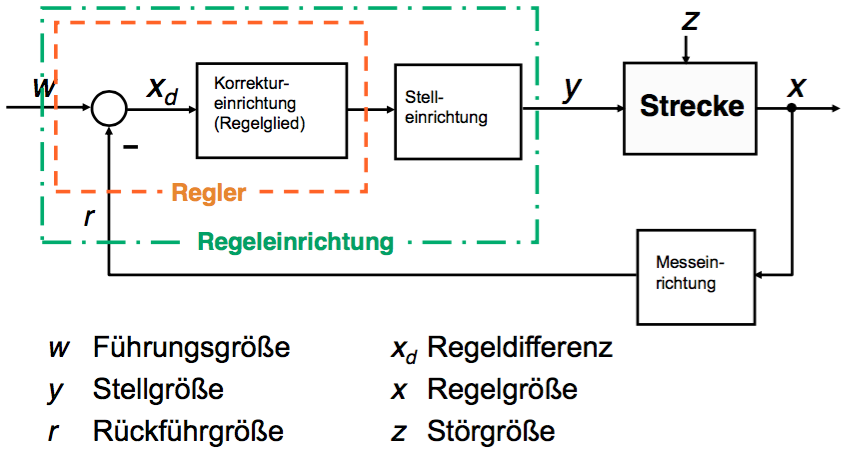
\includegraphics [scale=0.5]{regelkreis}
    \caption{Struktur eines Regelkreises}
\end{figure}

\mparagraph{Wirkungsweise}
\textbf{z} wird größer $\Rightarrow$ \textbf{x} wird gesenkt $\Rightarrow$ \textbf{r} wird abgesenkt
$\Rightarrow$ \textbf{$x_d$} wird angehoben $\Rightarrow$ \textbf{y} wird angehoben $\Rightarrow$
\textbf{x} wird angehoben mit der Tendenz den Sollwert \textbf{$x_s$} wieder anzunehmen. \\
Die Störgröße wird ausgeregelt.

\section{Grundlagen}
\subsection{Laplace Transformation}
\begin{compactitem}
    \item Rechenvereinfachung: Differential und Integralausdrücke werden zu algebraischen Ausdrücken.
    \item Gleichungslösung im Frequenzbereich statt Zeitbereich
    \item Integral muss konvergieren $\rightarrow$ lineare $f(t)$
\end{compactitem}
\begin{displaymath}
     L[f(t)] = f(s) = \int_0^\infty f(t)e^{-st}dt, s := \sigma + j\omega \text{ in } C \text{  } f(t)
      = 0, t < 0
\end{displaymath}

\begin{compactitem}
    \item \textbf{Linearitätssatz}: $L[\alpha f_i(t) + \beta f_2(t)] = \alpha f_1(s) + \beta f_2(s)$
    \item \textbf{Faltungssatz}: $L[f_1(t) * f_2(t)] = f_1(s) * f_2(s)$
    \item \textbf{Grenzwertsatz}: $f_1(t = 0) = \lim_{s \rightarrow \infty} s * f(s)$
    \item \textbf{Differentiationssatz}: $L[\frac{d}{dt}f(t)] = sF(s)$
    \item \textbf{Integrationssatz}: $L[\int f(t)dt] = \frac{1}{s}F(s)$

\end{compactitem}
\subsection{Übertragungsglieder}
\begin{compactitem}
    \item \textbf{P-Glied}: $y(t) = K * u(t)$
    \item \textbf{I-Glied}: $y(t) = K * \int_0^t u(\tau)d\tau$
    \item \textbf{D-Glied}: $y(t) = K * \dot{u}(t)$
    \item \textbf{T$_t$-Glied}: $y(t) = K * u(t-T_t)$
    \item \textbf{S-Glied}: $y(t) = K * \pm u_1(t) \pm u_2(t)$
    \item \textbf{KL-Glied}: $y(t) = K * F(u(t))$
    \item \textbf{M-Glied}: $y(t) = K * u_1(t)u_2(t)$
\end{compactitem}

\section{Reglertypen}
\subsection{PID Regler (und Unterklassen)}
\textbf{Sehr verbreitet, da für nahezu alle Prozesstypen geeignet, robust und mit geringem Aufwand
realisierbar} \\
P: güngstiges Regelverhalten, I: stationäre Genauigkeit, D: schnelle Ausregelung
\begin{align}
    u(t) = K_p (e(t) + \frac{1}{T_N}\int_o^t e(\tau)d\tau)+ T_V \frac{d}{dt}e(t))
\end{align}
mit Nachstellzeit $T_N$ und Vorhaltzeit $T_V$.

\mparagraph{Laplacetransformation}
\begin{align}
    u(t) &= K_Pe(t) + K_I \int e(t)dt + K_D \frac{d}{dt}e(t) \Leftrightarrow \\
    \Leftrightarrow u(s) &= K_Pe(s) + K_I \frac{1}{s}e(s) + K_Dse(s) \\
    \leftrightarrow \frac{u(s)}{e(s)} &= G(s) = K_P + K_I \frac{1}{s}+K_Ds \\
    \frac{\text{Ausgang}}{\text{Eingang}} &= \text{Übertragungsfunktion}
\end{align}
\subsection{Kennlinien- bzw. Kennlinienfeldregler}
\textbf{nihctlineare Übertragungsglieder}\\
z.B Zweipunktregler (Temperatur-Regelung)
\newpage
\subsection{Zustandsregler}
\textbf{Verbessertes Regelverhalten, da nicht nur die Regelabweichung, sondern im Idealfall alle
Zustandsgrößen der Regelstrecke zur Verfügung gestellt werden.} \\
regelungstechnische Behandlung von Mehrgrößensystemen, nichtlinearen und zeitvariablen
Übertragungssystemen.

\begin{figure}[!h]
    \centering
    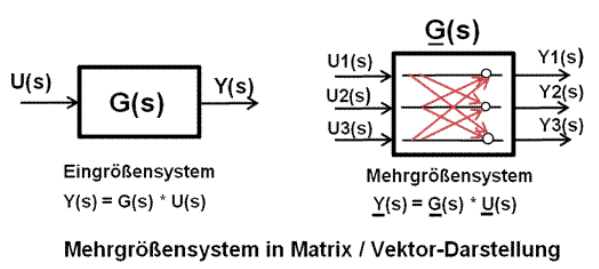
\includegraphics [scale=0.5]{mehrgroesse}
\end{figure}

\subsection{Kaskadenregelung}
\textbf{Unabhängige lineare Einzelregelkreis der einzelnen Gelenke}\\
Manipulator = Mehrgrößensystem

\begin{figure}[!h]
    \centering
    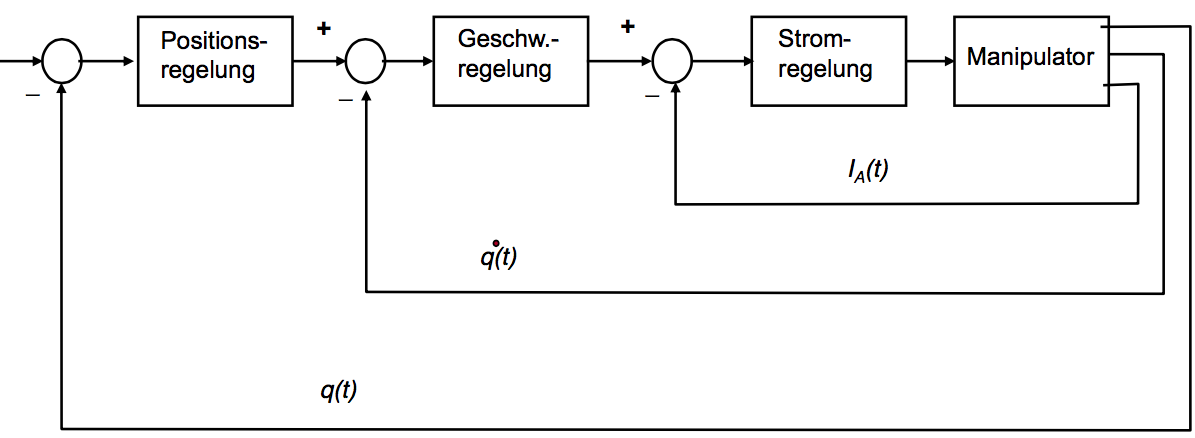
\includegraphics [scale=0.3]{kaskade}
\end{figure}

\subsection{Adaptive Regelung}
\textbf{Lageabhängige und somit zeitveränderliche Systemteile werden als Parameterschwankungen
aufgefasst}
\begin{figure}[!h]
    \centering
    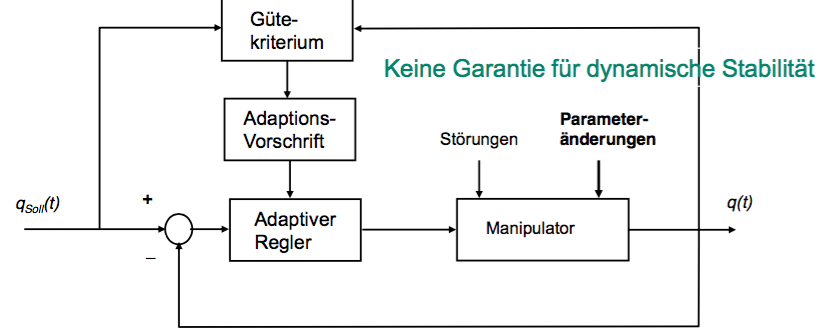
\includegraphics [scale=0.3]{adaptiv}
\end{figure}

\section{Regelungskonzepte für Manipulatoren}
\textbf{Regelung von Manipulatoren beschreibt nicht nur Positionsregelung, sondern auch die
Einbeziehung weiterer Umwelteinflüsste} (Massenträgheit des Manipulators, Gravitations-, Zentrifugal-,
Coriolis und Reibungskräfte/Momente auf die Gelenke)
\subsection{Exakte Systemmodellierung}
setzt a priori die exakte Kenntnis des Dynamikmodells und er Umgebung des Roboters voraus.
\subsection{Kraft-/Positionsregelung}
Position und Kräfte sind eng miteinander verknüpft. Steht Roboter in Kontakt mit Umgebung so bedeutet
Positionsänderung auch Kraftänderung und vice versa.

\mparagraph{Hybride Kraft-/Positionsregelung}
Wahlweise zwischen reiner Kraft und reiner Positionsregelung gewählt für jede kartesische Bewegungsrichtung
des Arms.
\mparagraph{Impedanz Regelung}
Regelt die dynamische Beziehung zwischen Kraft und Positions im Kontaktfall. \\
Idee: Interaktion Roboter-Umwelt verhält sich wie Feder-Dämpfer-Masse-System.
\begin{align}
     f(t) &= d * x(t)b * \dot{x}(t) + m * \ddot{x}(t)\\
     &\Rightarrow \text{Lapace Transformation} \Rightarrow \\
     F(s) &= (d + b+ s+ m *s ^2) * X(s)
\end{align}
Impedanz kann über Steifheit d, Dämpfung b und Trägheit m beeinflusst werden.

% !TEX root = rob1.tex
\chapter{Bahnsteuerung}




\end{document}
